\documentclass[a4paper,12pt]{article}
\usepackage{graphicx}
\usepackage{float}
\usepackage[english,russian]{babel}

\title{1.4.1 Изучение физического маятника}
\author{Тимур Байдюсенов Б01-302}
\date{29.09.2023}

\begin{document}
\maketitle

\section{Аннотация}
В работе определяется справедливость формул периода колебаний для физического маятника и значение g. Во время выполнения работы исследовалась зависимость периода колебаний физического маятника от его момента инерции. При обработке результатов оценил погрешность прямых и косвенных измерений.

\section{Теоретические сведения}
Физический маятник - любое твёрдое тело, которое под действием силы тяжести может свободно качатся вокруг неподвижной горизонтальной оси. Движение маятника описывается уравнением:
\begin{equation}
J\frac{d^2\varphi}{dt^2} = M
\end{equation}
где $J$ = момент инерции мятника, $\varphi$ - угол отклонения маятника от положения равновесия, $t$ - время, $M$ - момент сил, действующих на маятник

По теореме Гюйгенса-Штейнера момент инерции маятника вычисляется по формуле:
\begin{equation}
J = \frac{ml^2}{12}+ma^2
\end{equation}

Момент силы тяжести, действующий на маятник:
\begin{equation}
M = -mga\sin\varphi
\end{equation}
При малых углах $\varphi$ формула приобретает вид:
\begin{equation}
M \approx -mga\varphi
\end{equation}

Подставляя выражение для $J$ и $M$ в (1), получаем уравнениие:
\begin{equation}
\ddot{\varphi}+\omega^2\varphi=0
\end{equation}
где 
\begin{equation}
\omega^2 = \frac{ga}{a^2 + \frac{l^2}{12}}
\end{equation}

Период колебаний находится по формуле:
\begin{equation}
T = \frac{2\pi}{\omega} = 2\pi\sqrt{\frac{a^2 + \frac{l^2}{12}}{ag}}
\end{equation}

Период колебаний маятника без груза находится по формуле:
\begin{equation}
T = 2\pi\sqrt{\frac{\frac{l^2}{12} + a^2}{g(1 + \frac{m_{\mbox{пр}}}{m_{\mbox{ст}}})x_{\mbox{ц}}}}
\end{equation}

Период колебаний маятника с грузом находится по формуле:
\begin{equation}
T = 2\pi\sqrt{\frac{J_0 + m_{\mbox{г}}y^2}{gMx_{\mbox{ц}}}}
\end{equation}

\section{Оборудование}

\begin{figure}[H]
\begin{center}
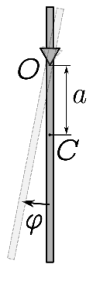
\includegraphics[width=0.2\textwidth]{маятник без груза}
\end{center}
\caption{А: Стержень как физический маятник}
\end{figure}

\begin{figure}[H]
\begin{center}
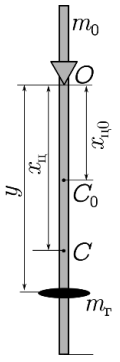
\includegraphics[width=0.2\textwidth]{маятник с грузом}
\end{center}
\caption{Б: Маятник с дополнительным грузом}
\end{figure}

Систематические погрешности приборов:

Штангенциркуль: $\Delta_{\mbox{шт}} = \pm 0.05$ мм

Линейка : $\Delta_{\mbox{л}} = \pm 0.5$ мм

Секундомер : $\Delta_{\mbox{с}} = \pm 0.005$ с

Весы : $\Delta_{\mbox{в}} = \pm 0.005$ г

\section{Результаты измерений и обработка данных}

Измерение оборудования:

$m_{\mbox{гр}} = 315,9$ г, масса груза

$m_{\mbox{ст}} = 890,8$ г, масса стержня

$m_{\mbox{пр}} = 76,0$ г, масса призмы

$l_{\mbox{ст}} = 996$ мм, длина стержня

\begin{table}[H]
\centering
\caption{Результаты измерения периода колебаний}
\begin{tabular}{|c|c|}
\hline
номер & t, с \\ \hline
1 & 30,75\\ \hline
2 & 30,75\\ \hline
3 & 30,70\\ \hline
4 & 30,72\\ \hline
5 & 30,77\\ \hline
6 & 30,70\\ \hline
7 & 30,71\\ \hline
8 & 30,74\\ \hline
9 & 30,73\\ \hline
10 & 30,74\\ \hline \hline
\overline{t}\mbox{, с} & 30,73\\ \hline
\sigma_{t}^{\mbox{случ}} & 0,025\\ \hline
\sigma_{t}^{\mbox{сист}} & 0,005\\ \hline
\sigma_{t}^{\mbox{полн}} & 0,026\\ \hline
\end{tabular}
\end{table}

Вычислим $\sigma_{t}^{\mbox{случ}}$ по формуле:

\begin{equation}
\sigma_{t}^{\mbox{случ}}=\sqrt{\frac{1}{N-1}\sum(t_i-\overline{t})^2}
\end{equation}

Вычислим $\sigma_{t}^{\mbox{полн}}$ по формуле:
\begin{equation}
\sigma_{t}^{\mbox{полн}}=\sqrt{\sigma_{t}^{\mbox{случ}}^2+\sigma_{t}^{\mbox{сист}}^2}
\end{equation}

Используя погрешность $\sigma_{t}$ измерения времени, оценим число колебаний $n$, по которому следует измерять период, чтобы относительная погрешность измерений была не хуже, чем $\epsilon \approx 0,1\%$

\begin{equation}
n=\frac{\sigma_{t}}{T\epsilon_T} = \frac{0,026} {1,5\cdot10^{-3}} \approx 17
\end{equation}

\begin{table}[H]
\centering
\caption{Результаты измерения периода для установки А(без груза)}
\begin{tabular}{|l|l|l|l|l|l|l|}
\hline
номер & a, м & $x_{\mbox{ц}}$, м & n & $t_n$, с & T, с & g, м/с\^2 \\ \hline
1 & 0,28 & 0,217 & 20 & 33,62 & 1,681 & 9,55\\ \hline
2 & 0,242 & 0,221 & 20 & 31,81 & 1,5905 & 10,47\\ \hline
3 & 0,253 & 0,234 & 20 & 32,67 & 1,6335 & 9,373\\ \hline
4 & 0,267 & 0,248 & 20 & 30,95 & 1,5475 & 9,85\\ \hline
5 & 0,249 & 0,232 & 20 & 31,38 & 1,569 & 10,24\\ \hline
6 & 0,256 & 0,237 & 20 & 32,46 & 1,623 & 9,37\\ \hline
7 & 0,263 & 0,244 & 20 & 31,21 & 1,5605 & 9,85\\ \hline
8 & 0,247 & 0,229 & 20 & 31,96 & 1,598 & 10,00\\ \hline
\end{tabular}
\end{table}

Для установки А вычислим g по формуле:
\begin{equation}
g = 4 \pi^{2} \frac{l^{2}/12 + a^{2}}{T^{2}x_{\mbox{ц}}(1+\frac{m_{\mbox{пр}}}{m_{\mbox{ст}}})}
\end{equation}

Определим погрешность по формуле:
\begin{eqnarray}
\sigma_{g} = 4\pi^{2} \sqrt{ (\frac{l}{6T^{2}x_{\mbox{ц}}(1+\frac{m_{\mbox{пр}}}{m_{\mbox{ст}}})}\sigma_{l})^{2} + (\frac{2a}{T^{2}x_{\mbox{ц}}(1+\frac{m_{\mbox{пр}}}{m_{\mbox{ст}}})}\sigma_{a})^{2} + (-2\frac{l^{2}/12 + a^{2}}{T^{3}x_{\mbox{ц}}(1+\frac{m_{\mbox{пр}}}{m_{\mbox{ст}}})} \sigma_{T})^{2}+}\nonumber \\
\overline{+ (-\frac{l^{2}/12 + a^{2}}{T^{2}x_{\mbox{ц}}^2(1+\frac{m_{\mbox{пр}}}{m_{\mbox{ст}}})}\sigma_{x_{\mbox{ц}}})^{2} + (-\frac{l^{2}/12 + a^{2}}{T^{2}x_{\mbox{ц}}}\frac{m_{\mbox{ст}}}{(m_{\mbox{пр}} + m_{\mbox{ст}})^2}\sigma_{m_{\mbox{пр}}})^{2}+}\nonumber \\
\overline{+ (\frac{l^{2}/12 + a^{2}}{T^{2}x_{\mbox{ц}}}\frac{m_{\mbox{пр}}}{(m_{\mbox{пр}} + m_{\mbox{ст}})^2}\sigma_{m_{\mbox{ст}}})^{2}}
\end{eqnarray}

Усредним значения $g$, получим: $g_{\mbox{a,ср}} = 9,84 \pm 0,07$ м/$c^2$


\begin{table}[H]
\centering
\caption{Результаты измерения периода для установки Б(с грузом)}
\begin{tabular}{|l|l|l|l|l|l|l|}
\hline
номер & y, м & $x_{\mbox{ц}}$, м & n & $t_n$, с & T, с & g, м/с\^2 \\ \hline
1 & 0,392 & 0,261 & 20 & 31,64 & 1,582 & 9,69\\ \hline
2 & 0,437 & 0,274 & 20 & 31,91 & 1,5955 & 10,18 \\ \hline
3 & 0,496 & 0,289 & 20 & 33,74 & 1,687 & 9,96 \\ \hline
4 & 0,606 & 0,315 & 20 & 37,05 & 1,8525 & 9,82 \\ \hline
5 & 0,579 & 0,31 & 20 & 36,64 & 1,832 & 9,62 \\ \hline
6 & 0,56 & 0,303 & 20 & 35,22 & 1,761 & 10,10 \\ \hline
7 & 0,53 & 0,296 & 20 & 34,33 & 1,7165 & 10,14 \\ \hline
8 & 0,596 & 0,306 & 20 & 36,61 & 1,8305 & 9,90 \\ \hline
\end{tabular}
\end{table}

Для установки Б вычислим g по формуле:
\begin{equation}
g = \frac{4\pi^{2}}{T^2} \frac{J_0 + m_{\mbox{г}}y^2}{Mx_{\mbox{ц}}}
\end{equation}
где $J_o = \frac{m_{\mbox{ст}}l_{\mbox{ст}}^2}{12} + m_{\mbox{ст}}a^2$

Усредним значения $g$, получим: $g_{\mbox{b,ср}} = 9,93\pm 0,07$ м/$c^2$

Построим график зависимости T(y):
\begin{figure}[H]
\begin{center}
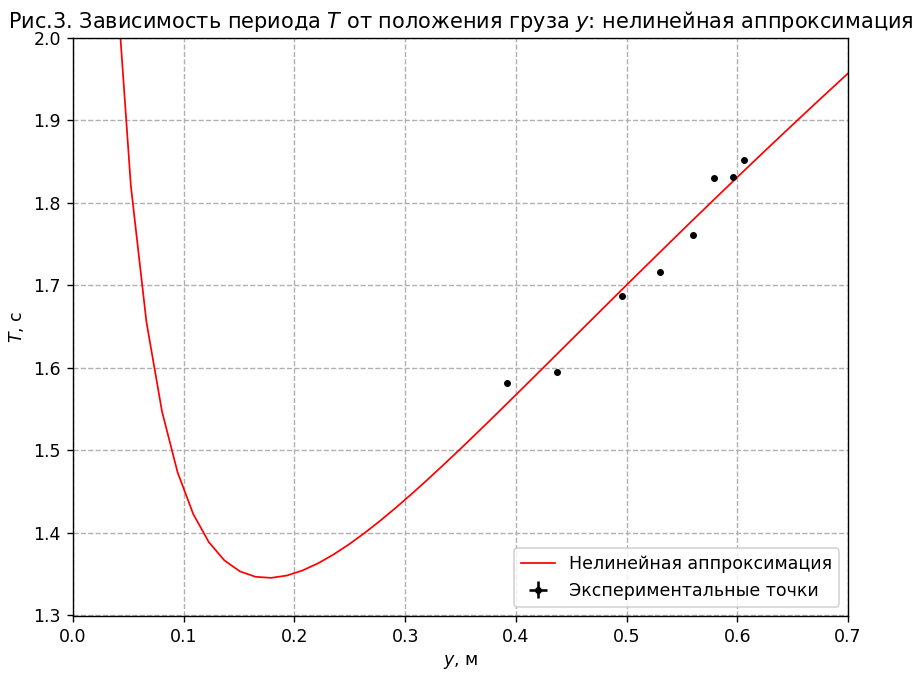
\includegraphics[width=1\textwidth]{T(a)}
\end{center}
\end{figure}

Найдем минимум с помощью графика:
\begin{figure}[H]
\begin{center}
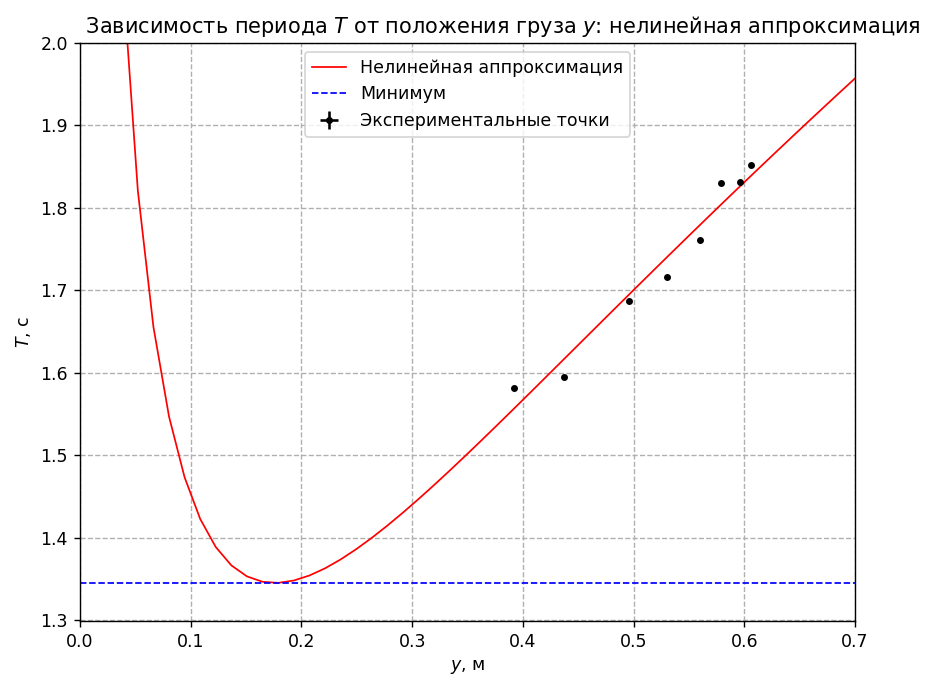
\includegraphics[width=1\textwidth]{T(a)+min}
\end{center}
\end{figure}

$T_{min} = 1,345 $ с согласно графику, что согласуется с теоретическим расчетом ($T_{min} = 1,52$ с). Однако измерение с помощью графика имеет существенную погрешность.

Построим график в координатах $u=T^2y$, $v = y^2$:
\begin{figure}[H]
\begin{center}
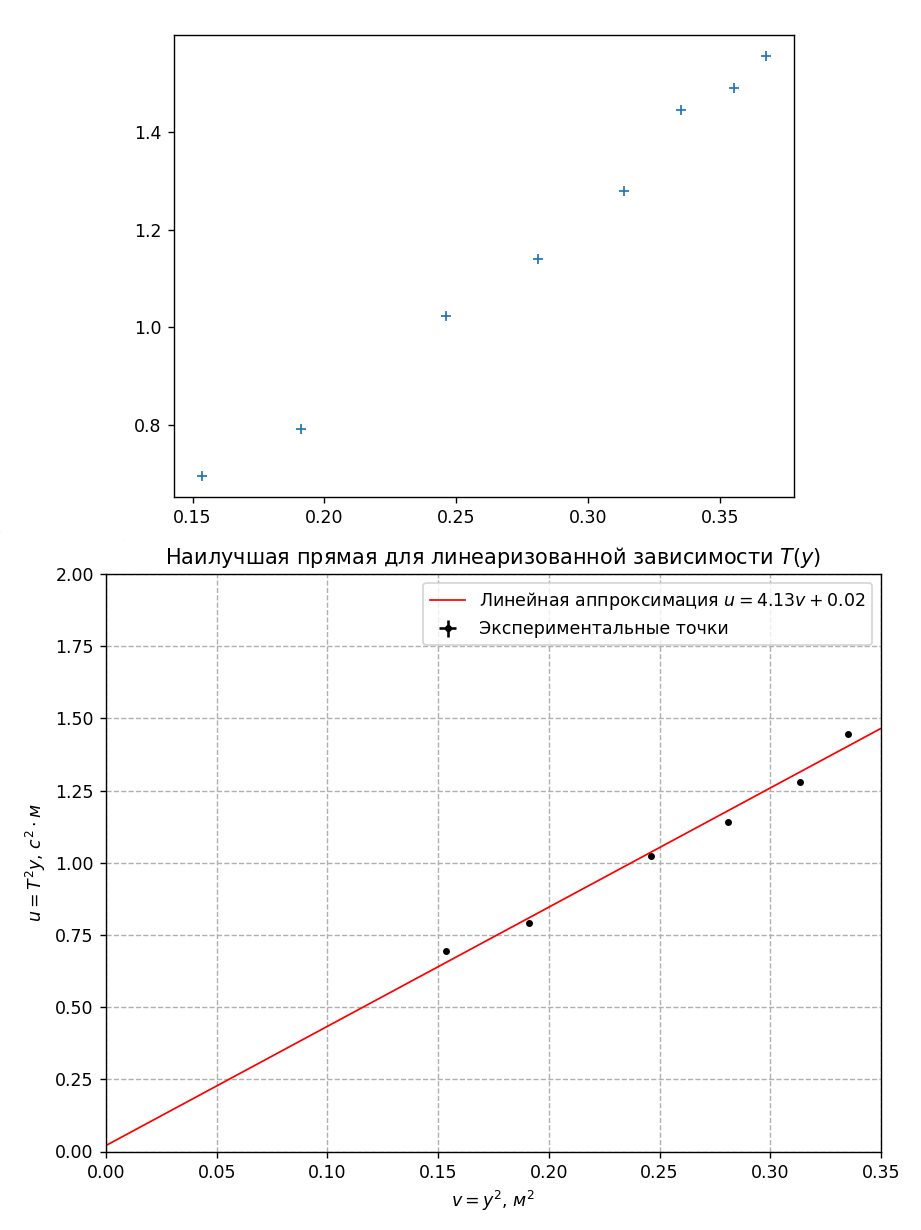
\includegraphics[width=1\textwidth]{U(v)}
\end{center}
\end{figure}

Определим $g$ с помощью графика, методом наименьших квадратов и оценим погрешность. В итоге получим, \[g=9,565 \pm 0,39 \mbox{ м/}c^2\]

\section{Вывод}
Определил справедливость формул периода колебаний для физического маятника и значение g. Во время выполнения работы исследовалал зависимость периода колебаний физического маятника от его момента инерции. При обработке результатов оценил погрешность прямых и косвенных измерений. В результате в обоих случаях были получены значения действительному: средее арифметическое: $g_{\mbox{b,ср}} = 9,93\pm 0,07 м/с^2$, по МНК: $g=9,565 \pm 0,39 \mbox{ м/}c^2$.

\end{document}
